In order to carry out a 3D mapping of the target, the system needs a light source to project points which will be used by the 3D mapping algorithm. In this section, the source of light will be designed.

\subsubsection{Design of the Light Source}
~\\
First of all, the green has been chosen as color of the light source. Indeed, in order to detect easily the points projected on the target, a distinctive color should be used. As we can see figure \ref{fig:QeCCD}, the CCD selected for the camera has the best quantum efficiency for a wavelength around 510 $nm$, which means that the green is the color that is the best recorded by the camera. Secondly, as the surface on Mars is mainly orange, red and brown, this color should stand out.


\begin{figure}[h]
  %\centering
  \centerline{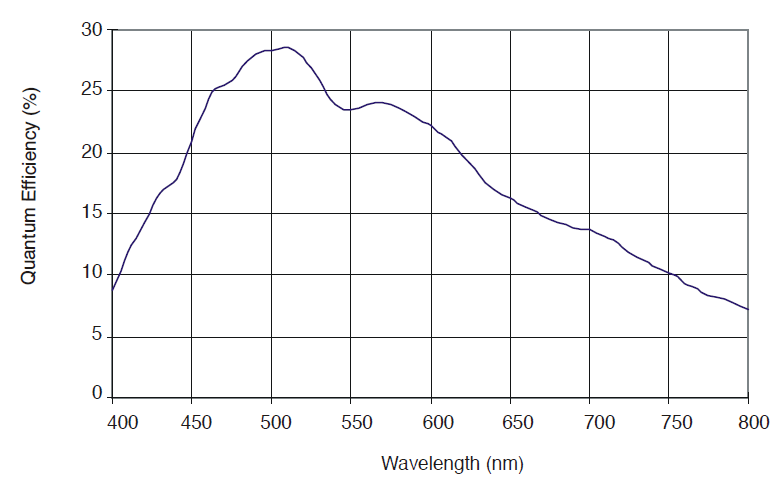
\includegraphics[scale=0.6]{fig/QeCCD.png}}
  \caption{Quantum efficiency versus wavelength of the CCD}
  \label{fig:QeCCD}
\end{figure}

Then, as only 300 $mW$ are available to aliment the light source and a lot of lightning energy is needed to outshine the sunlight, a LED has been chosen. Indeed, LEDs have great energy performances. The properties of the chosen LED can be seen in Annex \ref{LEDdatasheet}. Note that the use of a laser have been studied, but the energy cost would have been too expensive. Moreover, even if we cannot obtained a coherent light, as a laser do, with a LED, it is still feasible to obtain a monochromatic and directional light. Thus, we will assume that the LED can bring enough light (proof in part on Signal Noise Ratio\ref{light Power}).\
Then, as the 3D mapping algorithm needs a grid of points, the LED cannot be used in its present condition. Moreover, lot of light would be lost without an optic system. Thus, a system has been designed to concentrate the luminous beams of the LED and to transform the continuous light into a grid of point. The system uses a lens and a grid (Figure \ref{fig:LEDsystem}). 

\begin{figure}[h]
  %\centering
  \centerline{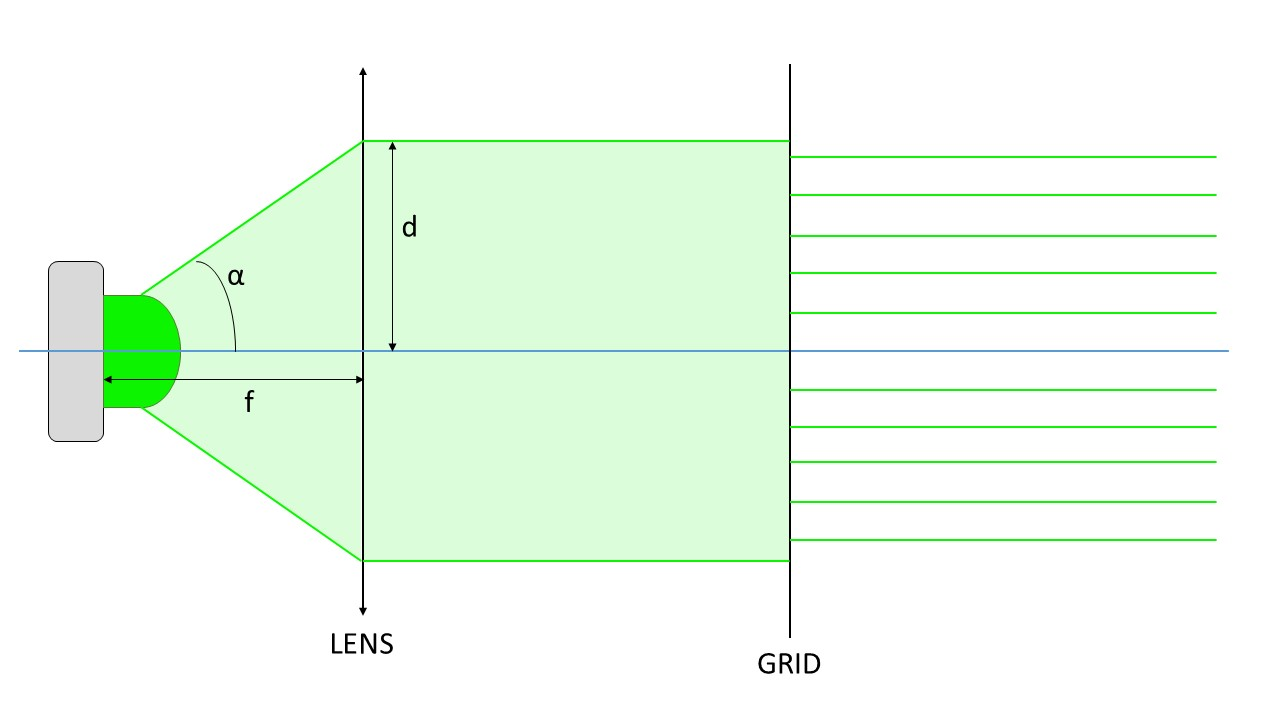
\includegraphics[scale=0.4]{fig/LEDsystem.jpg}}
  \caption{schema of the LED system}
  \label{fig:LEDsystem}
\end{figure}

As the LED has a diffusion angle of 30\textdegree (Annex \ref{LEDdatasheet}), the lens needs to be close enough to collect all the light beams of the LED to avoid losses of energy. In order to capture as much light as possible, the diameter of the lens should follow \eqref{eq:lenseLED}.

\begin{equation}
\label{eq:lenseLED}
d = f \tan \alpha
\end{equation}
with 
\begin{align*}
\alpha & = \frac{30}{2} = 15\mbox{\textdegree, the half of the diffusion angle.}\\
f & \mbox{, the focal length of the lens}
\end{align*}

Moreover, it should be pointed that there is a loss of energy because of the lens and the grid. We will assume that the energy loss coefficient of the lens $LFLLed$ (Loss Factor Lens Led) is 0.5 and the one of the grid $LFGLed$ (Loss Factor Grid Led) is 0.3.

\subsubsection{Validation of the Light Source}
\label{light Power}
~\\
In order to verify weather our light source has enough power or not to outshine the sunlight, the Signal/Noise ratio (SNR) has to be calculated (see part Signal/Noise ratio \ref{thirdcase}). Knowing that 100 is a really great SNR, as the SNR of images recorded with this system is $[32, 348]$, it can be concluded that the LED can be chosen as light source. Indeed, even if 32 is a low ratio, it is only when all the different poor conditions happen in the same time and it does not happen frequently. Moreover, 100 to 347are really high ratios that permit to have the 3D algorithm working well. Thus, the design of the light source is validated.




